\documentclass{article}


\usepackage{fancyhdr}
\usepackage{extramarks}
\usepackage{amsmath}
\usepackage{amsthm}
\usepackage{amsfonts}
\usepackage{tikz}
\usepackage[plain]{algorithm}
\usepackage{algpseudocode}
\usepackage{enumerate}
\usepackage{tikz}
\usepackage{listings}
\usepackage{hyperref}
\usepackage{subfigure}
\usepackage[graphicx]{realboxes}
\usepackage{xcolor}
\usepackage{color}



% 代码块高级设置
\lstset{
basicstyle=\footnotesize,                 % 设置整体的字体大小
showstringspaces=false,                     % 不显示字符串中的空格
frame=single,                               % 设置代码块边框
numbers=left,                               % 在左侧显示行号
% numberstyle=\footnotesize\color{gray},    % 设置行号格式
numberstyle=\color{darkgray},               % 设置行号格式
backgroundcolor=\color{white},              % 设置背景颜色
keywordstyle=\color{blue},                  % 设置关键字颜色
commentstyle=\it\color[RGB]{0,100,0},       % 设置代码注释的格式
stringstyle=\sl\color{red},                 % 设置字符串格式
}

\hypersetup{hidelinks,
	colorlinks=true,
	allcolors=black,
	pdfstartview=Fit,
	breaklinks=true}

%
% Basic Document Settings
%  

\topmargin=-0.45in
\evensidemargin=0in
\oddsidemargin=0in
\textwidth=6.5in
\textheight=9.0in
\headsep=0.25in

\linespread{1.1}

\pagestyle{fancy}
\lhead{}
\chead{\hmwkClass : \hmwkTitle}
\rhead{\firstxmark}
\lfoot{\lastxmark}
\cfoot{\thepage}

\renewcommand\headrulewidth{0.4pt}
\renewcommand\footrulewidth{0.4pt}

\setlength\parindent{0pt}



%
% Homework Details
%   - Title
%   - Due date
%   - Class
%   - Instructor
%   - Class number
%   - Name
%   - Student ID

\newcommand{\hmwkTitle}{Problem Set 4 Document}
\newcommand{\hmwkDueDate}{Dec 18th}
\newcommand{\hmwkClass}{Parallel Computing}
\newcommand{\hmwkClassInstructor}{Professor Rui Fan}

% 正式选课名单确定之后,根据通知填写所在班级编号

\newcommand{\hmwkAuthorName}{Zhenghong Yu}
\newcommand{\hmwkAuthorMail}{yuzhh1@shanghaitech.edu.cn}
\newcommand{\hmwkAuthorID}{2020533156}


%
% Title Page
%

\title{
    \vspace{2in}
    \textmd{\textbf{\hmwkClass:\\  \hmwkTitle}}\\
    \normalsize\vspace{0.1in}\small{Due\ on\ \hmwkDueDate\ at 23:59 }\\
   \vspace{2in}
}

\author{
    Mailbox: \hmwkAuthorMail\\
	Student ID: \hmwkAuthorID\\
    Student Name: \hmwkAuthorName}
\date{}




\begin{document}

\maketitle
\pagebreak
\tableofcontents

\pagebreak





\section{Problem 1}
Design a PRAM algorithm to compute an in-order traversal of a binary tree with 
$n$ nodes in $O(\log n)$ parallel time and $O(n)$ work.
\\\textbf{Solution: }\\
\begin{center}
    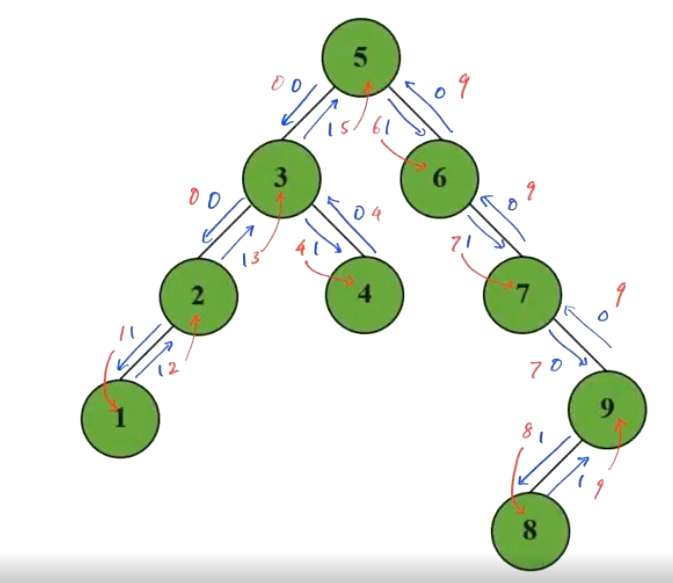
\includegraphics[scale = 0.3]{2.png}
\end{center}
Let $r$ be the root of the tree. First compute an Euler tour of the tree starting at $r$. Next, place values on each edge $(u,v)$ as follows:
\begin{itemize}
    \item If $(u,v)$ is a downwares edge(i.e. $u$ is the parent of $v$), then if $v$ does not have a left child, set $(u,v)$'s value to $1$ and otherwise set its value to $0$.
    \item If $(u,v)$ is an upwards edge(i.e. $v$ is the parent of $u$), then if $u$ is $v$'s left child, set $(u,v)$'s value to $1$, and otherwise set it to $0$.
\end{itemize} 
After setting the values, do a prefix sum on the linked list formed by the Euler tour. Finally, the in-order number of each node $v$ is defined as:
\begin{itemize}
    \item If $v$ has a left child $u$, then $v$'s value is the prefix sum value of edge $(u,v)$.
    \item If $v$ do not have a left child, then let $u$ be $v$'s parent. $v$'s value is the prefix sum value of $(u,v)$.
\end{itemize} 
Since we can compute the Euler tour, set the edge weights and assign edge prefix sum values to nodes in $O(1)$ time, and also prefix sum the edge weights in $O(\log n)$ time and $O(n)$ work, then the time complexity is $O(\log n)$ and the work is $O(n)$.

\section{Problem 2}
Design a PRAM algorithm to compute a histogram of a size $n$ array in $O(\log n)$
parallel time and $O(n)$ work. Assume all the values in the array are integers in 
the range 1 to $k= O(\log n)$. The output of the algorithm should be an array of
size $k$, where the $i$'th entry is the number of occurrences of value $i$.
\\\textbf{Solution: }\\
Let $k=O(\log n)$ be the number of different values in the array A. It's easy to solve the problem using $kn$ processors in $O(\log n)$ time and $O(nk)$ work as follows:
\begin{itemize}
    \item Assign one processor to each pair $(i,v)$, where $1\leq i\leq n$ is an index in A and $1\leq v\leq k$ is one of the values.
    \item In parallel, each processor $(i,v)$ sets a value $sum[i,v]$ to $1$ if $A[i]=v$, otherwise set it to $0$.
    \item In parallel, for each $1\leq v\leq k$, do a parallel sum reduction on $sum[1,v],sum[2,v],\cdots,sum[n,v]$. Set the histogram value for $v$ equal to the sum.  
\end{itemize} 
To make this algorithm more efficient (i.e. do $O(n)$ work), we use accelerate cascading. Specifically, we do the following,
\begin{itemize}
    \item Partiton A into $m=n/k$ chunks each of size $k$. Assign one processor to each pair $(i,v)$, where $1\leq i\leq m$ is the index of a chunk, and $1\leq v\leq k$ is one of the values. Notice that we use $O(n)$ processors.
    \item In parallel, each processor $(i,v)$ sequentially computes a histogram $H_{i}$ for all the values in its chunk of A in $O(k)$ time.
    \item Let C be an $m*k$ matrix where $i$th row is equal to $H_{i}$, for $1\leq i\leq m$.
    \item Using $n$ processors, do a parallel sum reduction on each column of C in parallel, to produce a size $k$ array that's the final histogram.    
\end{itemize} 
Step(b) takes $O(k)=O(\log n)$ parallel time and $O(n)$ work, Step(d) also takes $O(\log n)$ parallel time and $O(n)$ work. 
\begin{center}
    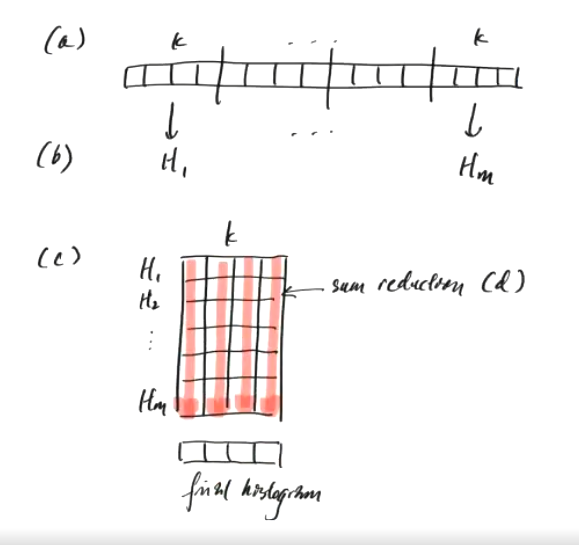
\includegraphics[scale = 0.3]{3.png}
\end{center}

\section{Problem 3}
Design a PRAM algorithm to implement Quicksort. What is the (expected) time 
and work complexity of your algorithm?
\\\textbf{Solution: }\\
The main step in Quicksort is to take an array and split it using a pivot value $v$ into a left part containing all values $\leq v$, and a right part containing all the values $>v$. This can be done in a way similar to sort on a single digit in radix sort in$O(\log n)$ time and $O(n)$ work. If we pick the pivots randomly, then Quicksort's recursion tree has $O(\log n)$ depth with high probability, and each level of the tree does $O(n)$ work in total. Thus, the total expected parallel time is $O(log^2 n)$ and the total work is $O(n\log n)$.






\end{document}
